\chapter{Porovnávání dvou překladů}
\label{chap:compare}

Při zobrazování rozdílů dvou překladů mohou být zvýrazněna slova či slovní spojení,
  která byla přeložena správně (potvrzené n-gramy),
  nebo která zlepšila či zhoršila překlad.

Druhou možností pro porovnávání překladů je zobrazení rozdílů porovnávaného překladu s referencí.
Pomocí této volby můžeme odhalit n-gramy,
  které se nacházejí na špatných pozicích ve větě,
  což může být způsobeno špatným slovosledem v překladu.

Při hledání potvrzených, zlepšujících n-gramů, zhoršujících n-gramů nebo zobrazování diffu můžeme narazit na několik problémů,
  které si vysvětlíme v následující kapitole.

\section{Hledání potvrzených n-gramů}
Jelikož se ve větách mohou slova či tokeny libovolně opakovat,
  můžeme narazit na situaci,
  kdy budeme mít více kandidátů na potvrzený n-gram.
Člověk snadno rozezná,
  který n-gram je potvrzený,
  ale v dlouhých větách by to mohlo být časově náročné,
  proto jsme chtěli najít algoritmus,
  který by ze všech kandidátů na potvrzený n-gram našel ty,
  které jsou s největší pravděpodobností potvrzené n-gramy.

Pro znázornění hledání potvrzených n-gramů je použit graf reprezentující porovnání dvou vět.
Tento graf se používá i pro výpočtu diffu nebo LCS,
  které později budeme používat.
Každá hrana v tomto grafu odpovídá jednomu slovu z porovnávaných vět.
Horizontální čáry v grafu reprezentují slova, která jsou v překladu navíc oproti referenci. 
Pro vertikální čáry to platí naopak, t.j. reprezentují slova, která jsou v referenci navíc oproti překladu.
Diagonální čáry reprezentují shodu mezi referencí a překladem.
Kandidáty na potvrzený n-gram mohou být reprezentováni jako diagonální hrany v grafu,
  který představuje porovnání dvou vět.
Ukázkový graf je možné vidět na Obrázku \ref{img:graph-1}.

\begin{figure}[h!]
	\centering
	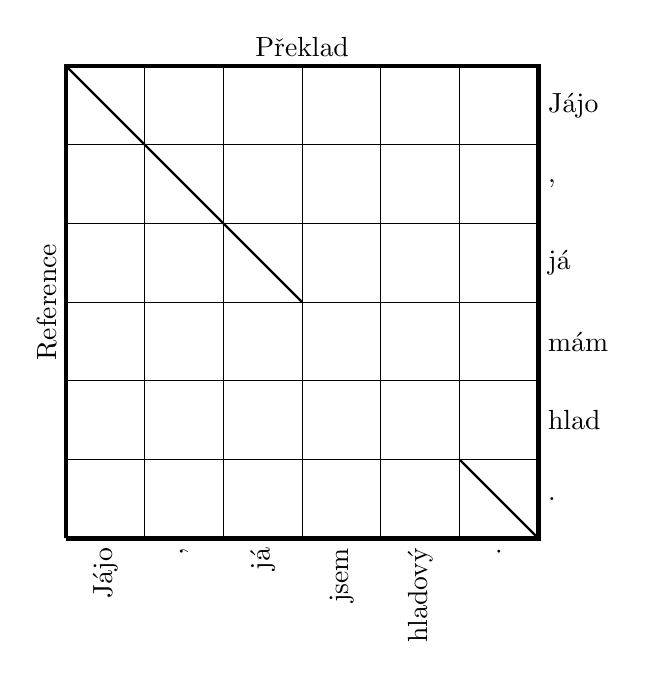
\begin{tikzpicture}
	  \draw [ ultra thick ] (0,0)--(0,6)--(6,6)--(6,0)--(0,0);
	  \draw (0,6)--(6,6) node [ midway, above ] { Překlad };
	  \draw (0,0)--(0,6) node [ midway, above, rotate=90] { Reference };

	  \draw (6,6)--(6,5) node [ midway, right ] { Jájo };
	  \draw (6,5)--(6,4) node [ midway, right ] {,};
	  \draw (6,4)--(6,3) node [ midway, right ] {já};
	  \draw (6,3)--(6,2) node [ midway, right ] {mám};
	  \draw (6,2)--(6,1) node [ midway, right ] {hlad};
	  \draw (6,1)--(6,0) node [ midway, right ] {.};

	  \draw (0,0)--(1,0) node [ midway, left, rotate=90] {Jájo};
	  \draw (1,0)--(2,0) node [ midway, left, rotate=90] {,};
	  \draw (2,0)--(3,0) node [ midway, left, rotate=90] {já};
	  \draw (3,0)--(4,0) node [ midway, left, rotate=90] {jsem};
	  \draw (4,0)--(5,0) node [ midway, left, rotate=90] {hladový};
	  \draw (5,0)--(6,0) node [ midway, left, rotate=90] {.};

	  \draw (0,1)--(6,1);
	  \draw (0,2)--(6,2);
	  \draw (0,3)--(6,3);
	  \draw (0,4)--(6,4);
	  \draw (0,5)--(6,5);
	  \draw (0,6)--(6,6);
	  \draw (1,0)--(1,6);
	  \draw (2,0)--(2,6);
	  \draw (3,0)--(3,6);
	  \draw (4,0)--(4,6);
	  \draw (5,0)--(5,6);

	  \draw [thick] (0,6)--(3,3);
	  \draw [thick] (5,1)--(6,0);
	\end{tikzpicture}

	\caption{
		Ukázka grafu porovnání dvou vět. \\
		\textbf{Reference}: Jájo, já mám hlad. \\
		\textbf{Překlad}: Jájo, já jsem hladový.
	}
	\label{img:graph-1}
\end{figure}

V případě,
  že počet kandidátů na potvrzený n-gram je stejný jako počet potvrzených n-gramů,
  je řešení našeho problému jednoduché.
V grafu to odpovídá situaci,
  kdy se v řádku a sloupci nachází stejný počet diagonálních čar.
V případě,
  že se nějaký potvrzený n-gram vyskytuje vícekrát,
  je vždy použit první ještě nepoužitý kandidát.
Všichni kandidáti na potvrzený n-gram jsou potvrzené n-gramy,
  a tak je můžeme patřičně zvýraznit.
Ve všech obrázcích budou potvrzené n-gramy zvýrazněny červenou barvou (to je možné vidět na Obrázku \ref{img:graph-2}).

\begin{figure}[h!]
	\centering
	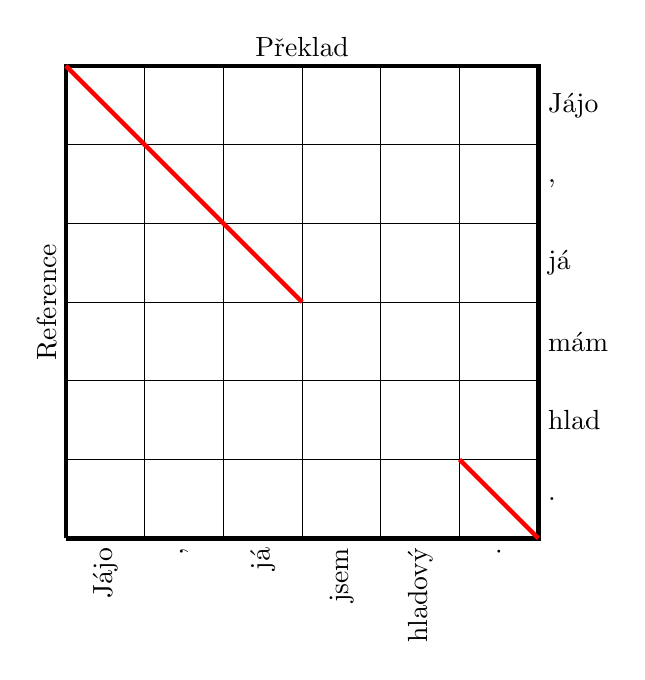
\begin{tikzpicture}
	  \draw [ ultra thick ] (0,0)--(0,6)--(6,6)--(6,0)--(0,0);
	  \draw (0,6)--(6,6) node [ midway, above ] { Překlad };
	  \draw (0,0)--(0,6) node [ midway, above, rotate=90] { Reference };

	  \draw (6,6)--(6,5) node [ midway, right ] { Jájo };
	  \draw (6,5)--(6,4) node [ midway, right ] {,};
	  \draw (6,4)--(6,3) node [ midway, right ] {já};
	  \draw (6,3)--(6,2) node [ midway, right ] {mám};
	  \draw (6,2)--(6,1) node [ midway, right ] {hlad};
	  \draw (6,1)--(6,0) node [ midway, right ] {.};

	  \draw (0,0)--(1,0) node [ midway, left, rotate=90] {Jájo};
	  \draw (1,0)--(2,0) node [ midway, left, rotate=90] {,};
	  \draw (2,0)--(3,0) node [ midway, left, rotate=90] {já};
	  \draw (3,0)--(4,0) node [ midway, left, rotate=90] {jsem};
	  \draw (4,0)--(5,0) node [ midway, left, rotate=90] {hladový};
	  \draw (5,0)--(6,0) node [ midway, left, rotate=90] {.};

	  \draw (0,1)--(6,1);
	  \draw (0,2)--(6,2);
	  \draw (0,3)--(6,3);
	  \draw (0,4)--(6,4);
	  \draw (0,5)--(6,5);
	  \draw (0,6)--(6,6);
	  \draw (1,0)--(1,6);
	  \draw (2,0)--(2,6);
	  \draw (3,0)--(3,6);
	  \draw (4,0)--(4,6);
	  \draw (5,0)--(5,6);

	  \draw [ultra thick, red] (0,6)--(3,3);
	  \draw [ultra thick, red] (5,1)--(6,0);
	\end{tikzpicture}

	\caption{
		Ukázka grafu porovnání dvou vět se zvýrazněnými potvrzenými n-gramy. \\
		\textbf{Reference}: Jájo, já mám hlad. \\
		\textbf{Překlad}: Jájo, já jsem hladový.
	}
	\label{img:graph-2}
\end{figure}

Těžší situace nastane,
  když je kandidátů na potvzený n-gram více než výskytů daného n-gramů v referenci.
Pro lepší představu je možné se podívat na Obrázek \ref{img:graph-3}.

\begin{figure}[h!]
	\centering
	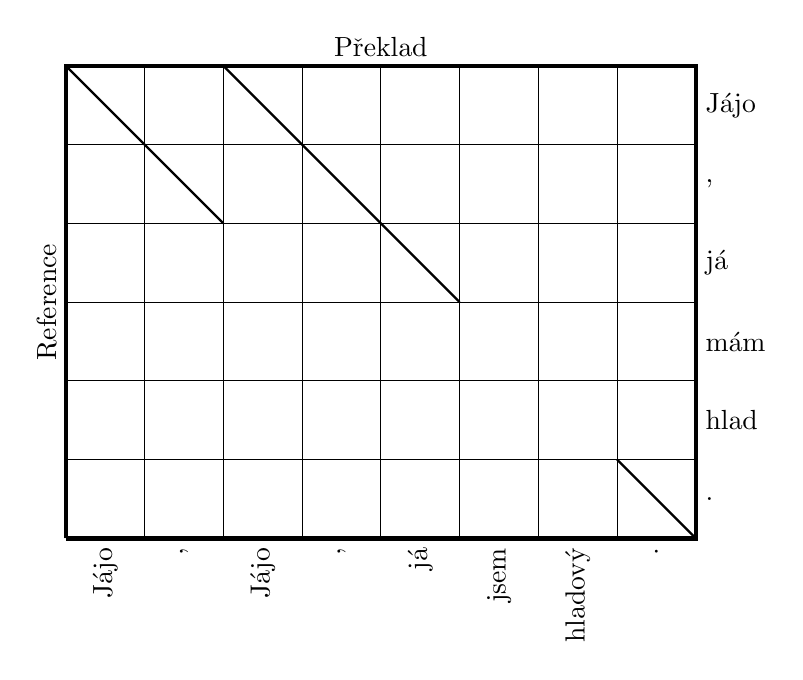
\begin{tikzpicture}
	  \draw [ ultra thick ] (0,0)--(0,6)--(8,6)--(8,0)--(0,0);
	  \draw (0,6)--(8,6) node [ midway, above ] { Překlad };
	  \draw (0,0)--(0,6) node [ midway, above, rotate=90] { Reference };

	  \draw (8,6)--(8,5) node [ midway, right ] { Jájo };
	  \draw (8,5)--(8,4) node [ midway, right ] {,};
	  \draw (8,4)--(8,3) node [ midway, right ] {já};
	  \draw (8,3)--(8,2) node [ midway, right ] {mám};
	  \draw (8,2)--(8,1) node [ midway, right ] {hlad};
	  \draw (8,1)--(8,0) node [ midway, right ] {.};

	  \draw (0,0)--(1,0) node [ midway, left, rotate=90] {Jájo};
	  \draw (1,0)--(2,0) node [ midway, left, rotate=90] {,};
	  \draw (2,0)--(3,0) node [ midway, left, rotate=90] {Jájo};
	  \draw (3,0)--(4,0) node [ midway, left, rotate=90] {,};
	  \draw (4,0)--(5,0) node [ midway, left, rotate=90] {já};
	  \draw (5,0)--(6,0) node [ midway, left, rotate=90] {jsem};
	  \draw (6,0)--(7,0) node [ midway, left, rotate=90] {hladový};
	  \draw (7,0)--(8,0) node [ midway, left, rotate=90] {.};

	  \draw (0,1)--(8,1);
	  \draw (0,2)--(8,2);
	  \draw (0,3)--(8,3);
	  \draw (0,4)--(8,4);
	  \draw (0,5)--(8,5);
	  \draw (0,6)--(8,6);
	  \draw (1,0)--(1,6);
	  \draw (2,0)--(2,6);
	  \draw (3,0)--(3,6);
	  \draw (4,0)--(4,6);
	  \draw (5,0)--(5,6);
	  \draw (6,0)--(6,6);
	  \draw (7,0)--(7,6);

	  \draw [thick] (0,6)--(2,4);
	  \draw [thick] (2,6)--(5,3);
	  \draw [thick] (7,1)--(8,0);
	\end{tikzpicture}

	\caption{
		Ukázka grafu s referencí a překladem, ve kterém se nachází více kandidátů pro n-gram \uv{Jájo,}. \\
		\textbf{Reference}: Jájo, já mám hlad. \\
		\textbf{Překlad}: Jájo, Jájo, já jsem hladový.
	}
	\label{img:graph-3}
\end{figure}

To je poměrně častý jev,
  který je k vidění např. u předložek, spojek nebo interpunkce.
V takovéto situaci by měly být vybrány takoví kandidáti,
  kteří se nacházejí v nejdelších možných potvrzených n-gramech.
K hledaní kandidátů nacházejících se v nejdelších potvrzených n-gramech je možné použít algoritmus pro hledání nejdelší společné podposloupnosti(LCS).
Nejdelší společná podposloupnost leží na nejkratší monotónní cestě v grafu,
  která vede z levého horního do pravého dolního rohu.
V obrázku budeme znázorňovat tuto cestu zelenou barvou.
Všichni kandidáti, kteří se nacházejí na této cestě,
  vždy patří mezi potvrzené n-gramy.
Výsledek použití algoritmu pro hledání nejdelší společné cesty je možné vidět na Obrázku \ref{img:graph-4}.

\begin{figure}[h!]
	\centering
	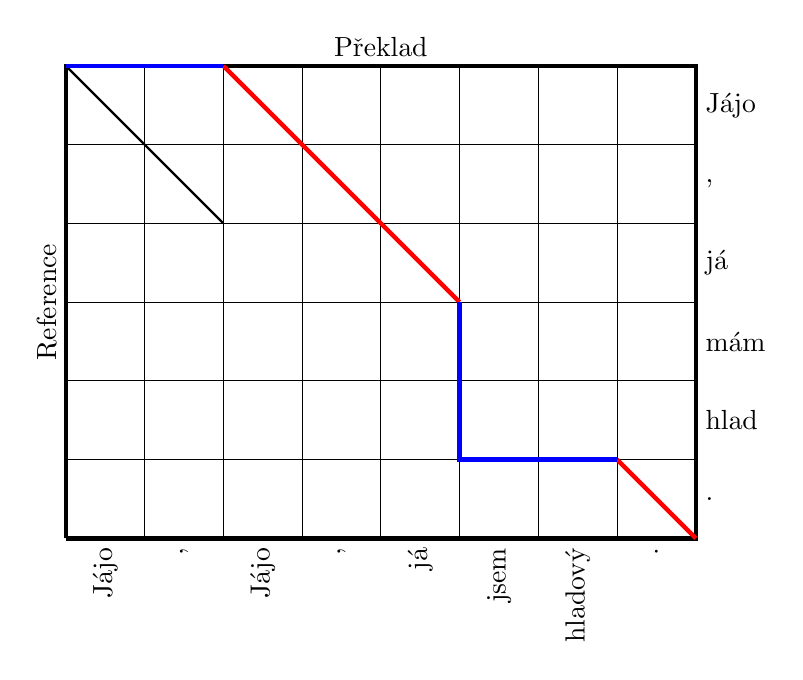
\begin{tikzpicture}
	  \draw [ ultra thick ] (0,0)--(0,6)--(8,6)--(8,0)--(0,0);
	  \draw (0,6)--(8,6) node [ midway, above ] { Překlad };
	  \draw (0,0)--(0,6) node [ midway, above, rotate=90] { Reference };

	  \draw (8,6)--(8,5) node [ midway, right ] { Jájo };
	  \draw (8,5)--(8,4) node [ midway, right ] {,};
	  \draw (8,4)--(8,3) node [ midway, right ] {já};
	  \draw (8,3)--(8,2) node [ midway, right ] {mám};
	  \draw (8,2)--(8,1) node [ midway, right ] {hlad};
	  \draw (8,1)--(8,0) node [ midway, right ] {.};

	  \draw (0,0)--(1,0) node [ midway, left, rotate=90] {Jájo};
	  \draw (1,0)--(2,0) node [ midway, left, rotate=90] {,};
	  \draw (2,0)--(3,0) node [ midway, left, rotate=90] {Jájo};
	  \draw (3,0)--(4,0) node [ midway, left, rotate=90] {,};
	  \draw (4,0)--(5,0) node [ midway, left, rotate=90] {já};
	  \draw (5,0)--(6,0) node [ midway, left, rotate=90] {jsem};
	  \draw (6,0)--(7,0) node [ midway, left, rotate=90] {hladový};
	  \draw (7,0)--(8,0) node [ midway, left, rotate=90] {.};

	  \draw (0,1)--(8,1);
	  \draw (0,2)--(8,2);
	  \draw (0,3)--(8,3);
	  \draw (0,4)--(8,4);
	  \draw (0,5)--(8,5);
	  \draw (0,6)--(8,6);
	  \draw (1,0)--(1,6);
	  \draw (2,0)--(2,6);
	  \draw (3,0)--(3,6);
	  \draw (4,0)--(4,6);
	  \draw (5,0)--(5,6);
	  \draw (6,0)--(6,6);
	  \draw (7,0)--(7,6);

	  \draw [thick] (0,6)--(2,4);
	  \draw [ultra thick, red] (2,6)--(5,3);
	  \draw [ultra thick, red] (7,1)--(8,0);

	  \draw [ultra thick, blue] (0,6)--(2,6);
		  \draw [ultra thick, blue] (5,3)--(5,1)--(7,1);
	\end{tikzpicture}

	\caption{Ukázka grafu s referencí a překladem, ve kterém se nachází více kandidátů pro n-gram \uv{Jájo,}.
		Zde je už zvýrazněna nejdelší společná podposloupnost, pomocí které je možné určit potvrzené n-gramy. \\
		\textbf{Reference}: Jájo, já mám hlad.\\
		\textbf{Překlad}: Jájo, Jájo, já jsem hladový.
	}
	\label{img:graph-4}
\end{figure}

Tímto postupem je možné nalézt pozice všech potvrzených n-gramů,
  které se nacházejí v nejdelší společné podposloupnosti.
Ale ne všechny potvrzené n-gramy se zde musí nacházet.
Například při změně pořadí slov v překladu se potvrzený n-gram nemusí nacházet v nejdelší společné podposloupnosti.
Tuto situaci ilustruje Obrázek \ref{img:graph-5}.

\begin{figure}[h!]
	\centering
	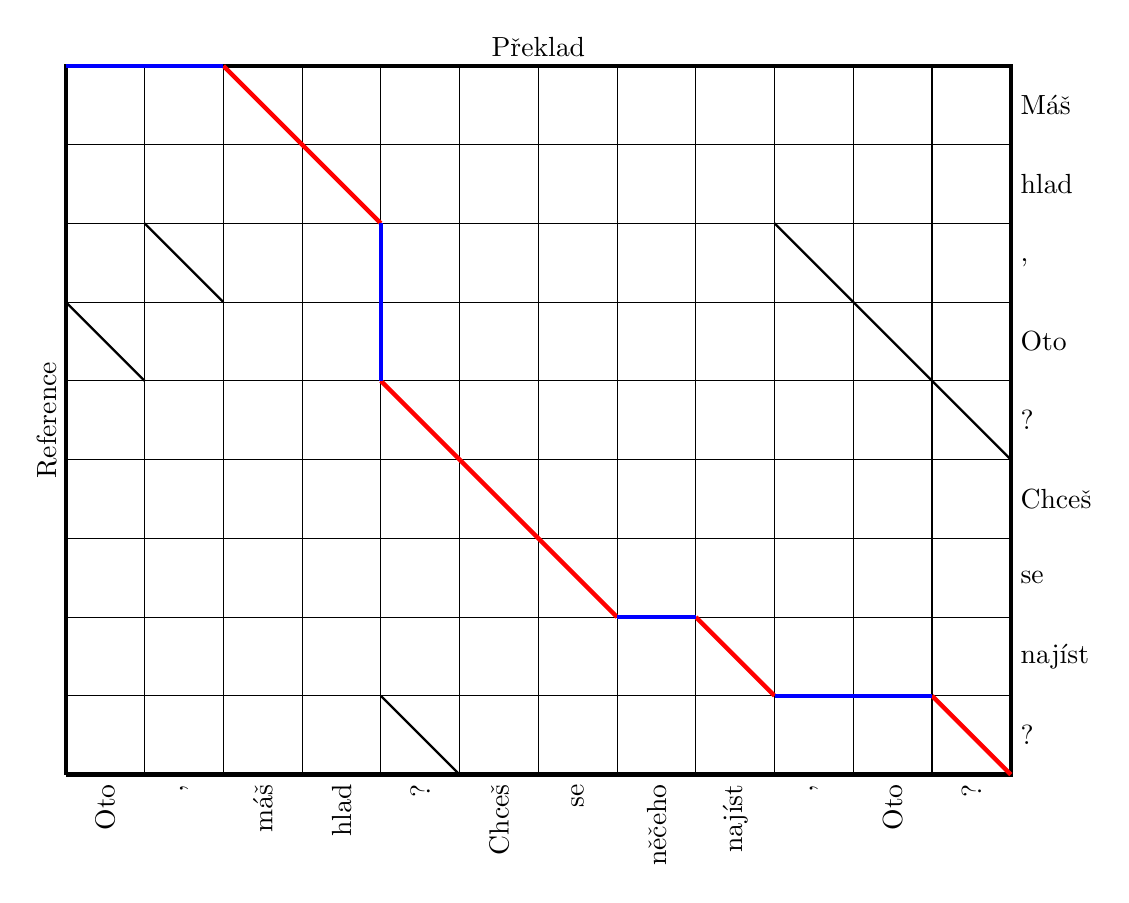
\begin{tikzpicture}
	  \draw [ ultra thick ] (0,0)--(0,9)--(12,9)--(12,0)--(0,0);
	  \draw (0,9)--(12,9) node [ midway, above ] { Překlad };
	  \draw (0,0)--(0,9) node [ midway, above, rotate=90] { Reference };

	  \draw (12,9)--(12,8) node [ midway, right ] {Máš};
	  \draw (12,8)--(12,7) node [ midway, right ] {hlad};
	  \draw (12,7)--(12,6) node [ midway, right ] {,};
	  \draw (12,6)--(12,5) node [ midway, right ] {Oto};
	  \draw (12,5)--(12,4) node [ midway, right ] {?};
	  \draw (12,4)--(12,3) node [ midway, right ] {Chceš};
	  \draw (12,3)--(12,2) node [ midway, right ] {se};
	  \draw (12,2)--(12,1) node [ midway, right ] {najíst};
	  \draw (12,1)--(12,0) node [ midway, right ] {?};

	  \draw (0,0)--(1,0) node [ midway, left, rotate=90] {Oto};
	  \draw (1,0)--(2,0) node [ midway, left, rotate=90] {,};
	  \draw (2,0)--(3,0) node [ midway, left, rotate=90] {máš};
	  \draw (3,0)--(4,0) node [ midway, left, rotate=90] {hlad};
	  \draw (4,0)--(5,0) node [ midway, left, rotate=90] {?};
	  \draw (5,0)--(6,0) node [ midway, left, rotate=90] {Chceš};
	  \draw (6,0)--(7,0) node [ midway, left, rotate=90] {se};
	  \draw (7,0)--(8,0) node [ midway, left, rotate=90] {něčeho};
	  \draw (8,0)--(9,0) node [ midway, left, rotate=90] {najíst};
	  \draw (9,0)--(10,0) node [ midway, left, rotate=90] {,};
	  \draw (10,0)--(11,0) node [ midway, left, rotate=90] {Oto};
	  \draw (11,0)--(12,0) node [ midway, left, rotate=90] {?};

	  \draw (0,1)--(12,1);
	  \draw (0,2)--(12,2);
	  \draw (0,3)--(12,3);
	  \draw (0,4)--(12,4);
	  \draw (0,5)--(12,5);
	  \draw (0,6)--(12,6);
	  \draw (0,7)--(12,7);
	  \draw (0,8)--(12,8);
	  \draw (0,9)--(12,9);
	  \draw (1,0)--(1,9);
	  \draw (2,0)--(2,9);
	  \draw (3,0)--(3,9);
	  \draw (4,0)--(4,9);
	  \draw (5,0)--(5,9);
	  \draw (6,0)--(6,9);
	  \draw (7,0)--(7,9);
	  \draw (8,0)--(8,9);
	  \draw (9,0)--(9,9);
	  \draw (10,0)--(10,9);
	  \draw (11,0)--(11,9);
	  \draw (12,0)--(12,9);

	  \draw [ultra thick, red] (2,9)--(4,7);
	  \draw [ultra thick, red] (4,5)--(7,2);
	  \draw [ultra thick, red] (8,2)--(9,1);
	  \draw [ultra thick, red] (11,1)--(12,0);

	  \draw [ultra thick, blue] (0,9)--(2,9);
	  \draw [ultra thick, blue] (4,7)--(4,5);
	  \draw [ultra thick, blue] (7,2)--(8,2);
	  \draw [ultra thick, blue] (9,1)--(11,1);


	  \draw [thick] (1,7)--(2,6);
	  \draw [thick] (0,6)--(1,5);
	  \draw [thick] (9,7)--(12,4);
	  \draw [thick] (4,1)--(5,0);


	\end{tikzpicture}

	\caption{
		Ukázka grafu s referencí a překladem, ve kterém se nachází více kandidátů pro n-gramy \uv{Oto} a \uv{,}. \\
		\textbf{Reference}: Máš hlad, Oto? Chceš se najíst?\\
		\textbf{Překlad}: Oto, máš hlad? Chceš se něčeho najíst, Oto?
	}
	\label{img:graph-5}
\end{figure}

I tato situace může nastat poměrně často,
  a proto musel být nalezen způsob,
  jak z kandidátů potvrzených n-gramů,
  kteří se nacházejí mimo nejdelší společnou podposloupnost,
  budou vybrány potvrzené n-gramy. 


Při vymýšlení algoritmu pro řešení této situace byl použit stejný předpoklad jako v minulém případě.
To je, že z kadidátů potvrzených n-gramů budou vybráni vždy ti kandidáti,
  kteří se nacházejí uvnitř nejdelších potvrzených n-gramů.
Každý token v překladu může být ohodnocen pomocí skóre,
  které určuje v kolika kandidátech potvrzených n-gramů a již potvrzených n-gramech se daný token nachází.
Z kadidátů na potvrzený n-gram pak jsou vybráni ti,
  kteří mají největší skóre celého n-gramu,
  které se spočítá jako součet skóre tokenů v n-gramu.
Aby dále nebyli zvýhodňováni kandidáti,
  kteří byli součástí delších nezvolených kandidátů,
  musí být po každé volbě potvrzených n-gramů upraveno skóre u tokenů patřících do kandidátů potvrzených,
  kteří nebyli zvoleni za potvrzené n-gramy.
Výsledek použítí tohoto algoritmu je zachycen na Obrázku \ref{img:graph-6}.

\begin{figure}[h!]
	\centering
	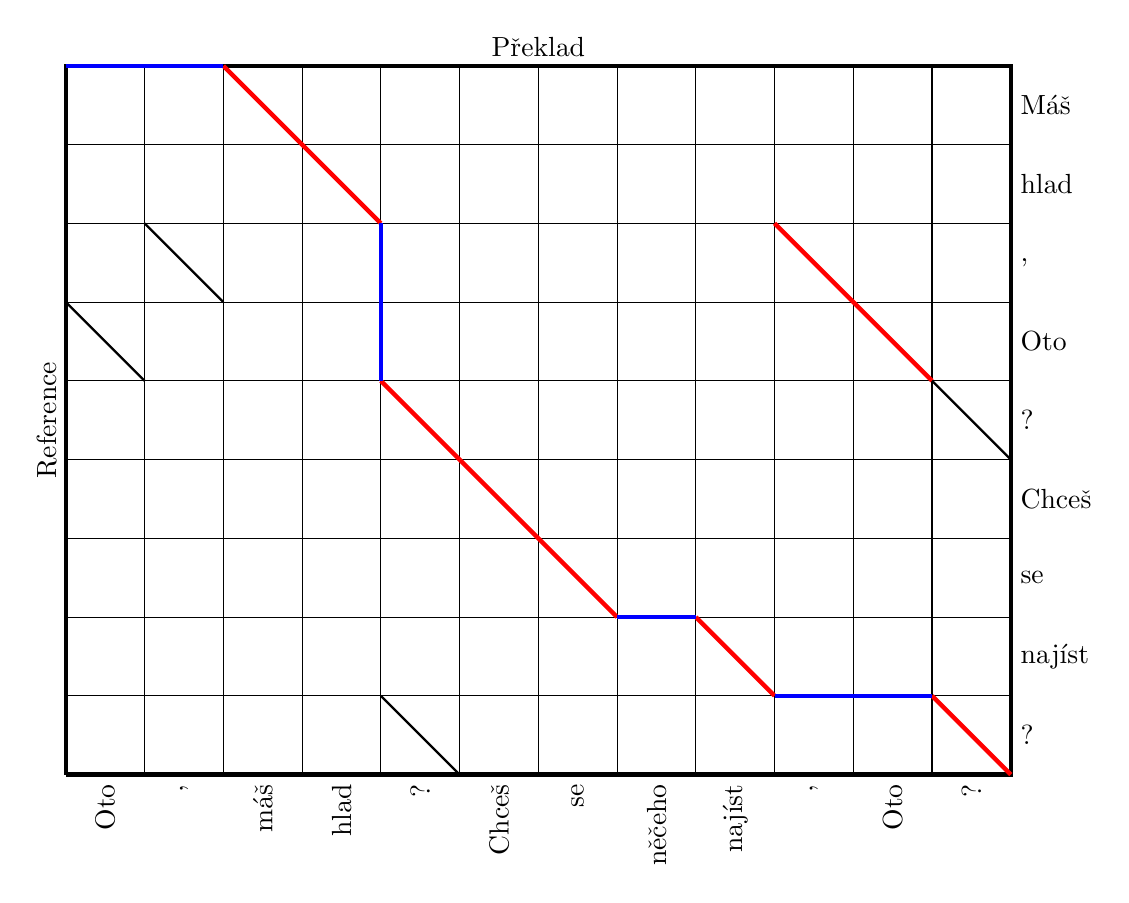
\begin{tikzpicture}
	  \draw [ ultra thick ] (0,0)--(0,9)--(12,9)--(12,0)--(0,0);
	  \draw (0,9)--(12,9) node [ midway, above ] { Překlad };
	  \draw (0,0)--(0,9) node [ midway, above, rotate=90] { Reference };

	  \draw (12,9)--(12,8) node [ midway, right ] {Máš};
	  \draw (12,8)--(12,7) node [ midway, right ] {hlad};
	  \draw (12,7)--(12,6) node [ midway, right ] {,};
	  \draw (12,6)--(12,5) node [ midway, right ] {Oto};
	  \draw (12,5)--(12,4) node [ midway, right ] {?};
	  \draw (12,4)--(12,3) node [ midway, right ] {Chceš};
	  \draw (12,3)--(12,2) node [ midway, right ] {se};
	  \draw (12,2)--(12,1) node [ midway, right ] {najíst};
	  \draw (12,1)--(12,0) node [ midway, right ] {?};

	  \draw (0,0)--(1,0) node [ midway, left, rotate=90] {Oto};
	  \draw (1,0)--(2,0) node [ midway, left, rotate=90] {,};
	  \draw (2,0)--(3,0) node [ midway, left, rotate=90] {máš};
	  \draw (3,0)--(4,0) node [ midway, left, rotate=90] {hlad};
	  \draw (4,0)--(5,0) node [ midway, left, rotate=90] {?};
	  \draw (5,0)--(6,0) node [ midway, left, rotate=90] {Chceš};
	  \draw (6,0)--(7,0) node [ midway, left, rotate=90] {se};
	  \draw (7,0)--(8,0) node [ midway, left, rotate=90] {něčeho};
	  \draw (8,0)--(9,0) node [ midway, left, rotate=90] {najíst};
	  \draw (9,0)--(10,0) node [ midway, left, rotate=90] {,};
	  \draw (10,0)--(11,0) node [ midway, left, rotate=90] {Oto};
	  \draw (11,0)--(12,0) node [ midway, left, rotate=90] {?};

	  \draw (0,1)--(12,1);
	  \draw (0,2)--(12,2);
	  \draw (0,3)--(12,3);
	  \draw (0,4)--(12,4);
	  \draw (0,5)--(12,5);
	  \draw (0,6)--(12,6);
	  \draw (0,7)--(12,7);
	  \draw (0,8)--(12,8);
	  \draw (0,9)--(12,9);
	  \draw (1,0)--(1,9);
	  \draw (2,0)--(2,9);
	  \draw (3,0)--(3,9);
	  \draw (4,0)--(4,9);
	  \draw (5,0)--(5,9);
	  \draw (6,0)--(6,9);
	  \draw (7,0)--(7,9);
	  \draw (8,0)--(8,9);
	  \draw (9,0)--(9,9);
	  \draw (10,0)--(10,9);
	  \draw (11,0)--(11,9);
	  \draw (12,0)--(12,9);

	  \draw [ultra thick, red] (2,9)--(4,7);
	  \draw [ultra thick, red] (4,5)--(7,2);
	  \draw [ultra thick, red] (8,2)--(9,1);
	  \draw [ultra thick, red] (11,1)--(12,0);
	  \draw [ultra thick, red] (9,7)--(11,5);

	  \draw [ultra thick, blue] (0,9)--(2,9);
	  \draw [ultra thick, blue] (4,7)--(4,5);
	  \draw [ultra thick, blue] (7,2)--(8,2);
	  \draw [ultra thick, blue] (9,1)--(11,1);


	  \draw [thick] (1,7)--(2,6);
	  \draw [thick] (0,6)--(1,5);
	  \draw [thick] (11,5)--(12,4);
	  \draw [thick] (4,1)--(5,0);


	\end{tikzpicture}

	\caption{
		Ukázka grafu s referencí a překladem, ve kterém se nachází více kandidátů pro n-gramy \uv{Oto} a \uv{,}.
		Pozice těchto n-gramů byla nalezena pomocí metody s počítáním skóre.
		I když nalezené pozice n-gramů \uv{Oto} a \uv{,} neodpovídají lidskému úsudku,
		jsou tyto pozice nalezené správně vzhledem k metrice BLEU. \\
		\textbf{Reference}: Máš hlad, Oto? Chceš se najíst?\\
		\textbf{Překlad}: Oto, máš hlad? Chceš se něčeho najíst, Oto?
	}
	\label{img:graph-6}
\end{figure}
  
Aby oba dva přístupy mohly být zkombinovány do jednoho algoritmu a
  jednotlivé případy nemuseli být řešeny odděleně,
  byla přídána bonifikace pro tokeny,
  které se nacházejí v nejdelší společné podposloupnosti reference a překladu.
Tyto tokeny budou mít vždy vyšší skóre než jejich konkurenti,
  a proto nemůže dojít k situaci,
  že by token ležící v nejdelší společené podposloupnosti nebyl částí potvrzeného n-gramu.
Nalezení potvrzených n-gramů pak může být provedeno pouze pomocí počítání skóre.


Avšak i kombinace těchto dvou přístupů nemusí vždy fungovat.
Jelikož tento algoritmus počítá pouze s n-gramy do délky čtyř tokenů,
  potvrzené n-gramy,
  které se nenacházejí v nejdelší společné podposloupnosti a jsou delší než sedm tokenů,
  nemusejí být správně označeny za potvrzené.
U takovýchto n-gramů záleží pouze na pořadí, v jakém se ve větě vyskytují.
Část n-gramu,
  který se ve větě vyskytne dříve,
  bude prohlášen za potvrzený n-gram.

V praxi se ale tyto případy moc nevyskytují -
  nestává se často, že by se ve větě nacházelo více kandidátů pro n-gram délky vyšší než sedm tokenů,
  proto by tento algoritmus měl ve většině případů fungovat dobře.


\section{Počítání diffu mezi dvěma překlady}
Pro počítání diffu mezi dvěma překlady může být použit stejný algoritmus,
  který byl použit k hledání nejdelší společné podposloupnosti dvou překladů.
Diff je stejně jako nejdelší společná podposloupnost reprezentován nejkratší monotonní cestou vedoucí z levého horního do pravého dolního rohu v grafu porovnání reference a překladu.
Změna je pouze v tom, že horizontální hrany ležící na této cestě odpovídají tokenům,
  které byly navíc vloženy do překladu.
V diagramu budou označeny modrou barvou.
Vertikální hrany ležící na cestě reprezentující nejdelší společnou podposloupnost odpovídají tokenům,
  které byly navíc vloženy do reference.
V diagramu budou označeny červenou barvou.
Diagonální hrany ležící na výše definované cestě reprezentují tokeny,
  které se nacházejí i v referenci i v překladu.
V diagramu budou označeny zelenou barvou.
Výsledek počítání diffu dvou vět ukazuje Obrázek \ref{img:graph-7}.
Z takto obarvené cesty může být zjištěn rozdíl mezi porovnávanými větami
  a na jeho základě může být zobrazen rozdíl ve webovém prostředí.

\begin{figure}[h!]
	\centering
	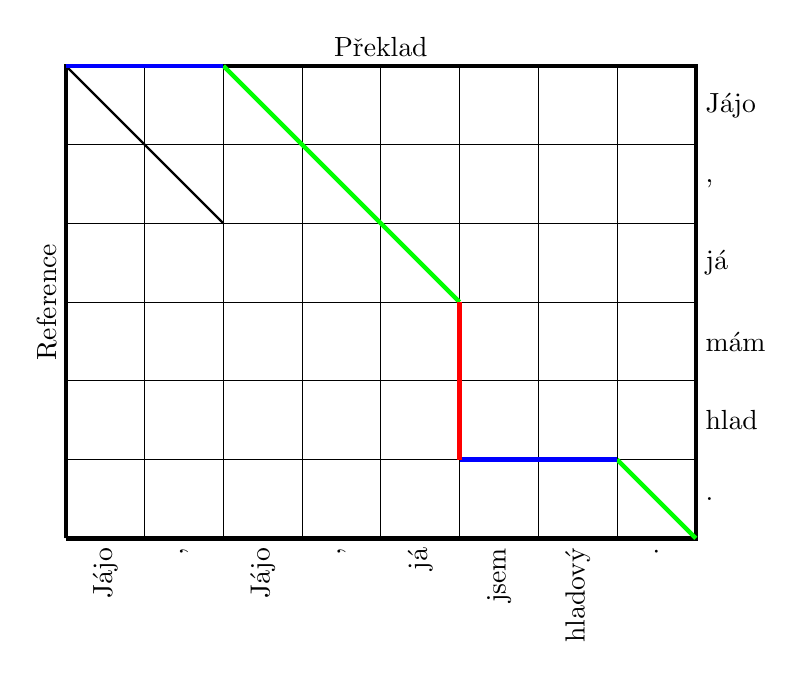
\begin{tikzpicture}
	  \draw [ ultra thick ] (0,0)--(0,6)--(8,6)--(8,0)--(0,0);
	  \draw (0,6)--(8,6) node [ midway, above ] { Překlad };
	  \draw (0,0)--(0,6) node [ midway, above, rotate=90] { Reference };

	  \draw (8,6)--(8,5) node [ midway, right ] { Jájo };
	  \draw (8,5)--(8,4) node [ midway, right ] {,};
	  \draw (8,4)--(8,3) node [ midway, right ] {já};
	  \draw (8,3)--(8,2) node [ midway, right ] {mám};
	  \draw (8,2)--(8,1) node [ midway, right ] {hlad};
	  \draw (8,1)--(8,0) node [ midway, right ] {.};

	  \draw (0,0)--(1,0) node [ midway, left, rotate=90] {Jájo};
	  \draw (1,0)--(2,0) node [ midway, left, rotate=90] {,};
	  \draw (2,0)--(3,0) node [ midway, left, rotate=90] {Jájo};
	  \draw (3,0)--(4,0) node [ midway, left, rotate=90] {,};
	  \draw (4,0)--(5,0) node [ midway, left, rotate=90] {já};
	  \draw (5,0)--(6,0) node [ midway, left, rotate=90] {jsem};
	  \draw (6,0)--(7,0) node [ midway, left, rotate=90] {hladový};
	  \draw (7,0)--(8,0) node [ midway, left, rotate=90] {.};

	  \draw (0,1)--(8,1);
	  \draw (0,2)--(8,2);
	  \draw (0,3)--(8,3);
	  \draw (0,4)--(8,4);
	  \draw (0,5)--(8,5);
	  \draw (0,6)--(8,6);
	  \draw (1,0)--(1,6);
	  \draw (2,0)--(2,6);
	  \draw (3,0)--(3,6);
	  \draw (4,0)--(4,6);
	  \draw (5,0)--(5,6);
	  \draw (6,0)--(6,6);
	  \draw (7,0)--(7,6);

	  \draw [thick] (0,6)--(2,4);
	  \draw [ultra thick, green] (2,6)--(5,3);
	  \draw [ultra thick, green] (7,1)--(8,0);

	  \draw [ultra thick, blue] (0,6)--(2,6);
	  \draw [ultra thick, blue] (5,1)--(7,1);

	  \draw [ultra thick, red] (5,3)--(5,1);
	\end{tikzpicture}

	\caption{
		Ukázka diffu reference s překladem. \\
		\textbf{Reference}: Jájo, já mám hlad.\\
		\textbf{Překlad}: Jájo, Jájo, já jsem hladový.
	}
	\label{img:graph-4}
\end{figure}
